\documentclass[onecolumn, oneside, letterpaper, draftclsnofoot, 10pt, compsoc]{IEEEtran}

\usepackage[english]{babel}
\usepackage{graphicx}
\usepackage{url}
\usepackage{setspace}
\usepackage{subcaption}

\usepackage{amssymb}
\usepackage{amsmath}
\usepackage{amsthm}
\usepackage{alltt}
\usepackage{color}
\usepackage{enumitem}
\usepackage{textcomp}
\usepackage{cite}
\usepackage{comment}

%\usepackage[T1]{fontenc}
\usepackage[utf8]{inputenc}
\usepackage{lmodern}
\usepackage[hidelinks]{hyperref}
\usepackage[normalem]{ulem}

\usepackage[margin=0.75in]{geometry}

\parindent = 0.0 in
\parskip = 0.0 in

% 1. Fill in these details
\def \CapstoneTeamName{         Beaver Hawks}
\def \CapstoneTeamNumber{       14}
\def \GroupMemberOne{           Anton Synytsia}
\def \GroupMemberTwo{           Matthew Phillips}
\def \GroupMemberThree{         Shanmukh Challa}
\def \GroupMemberFour{          Nathan Tan}
\def \CapstoneProjectName{      American Helicopter Society Micro Air Vehicle Competition}
\def \CapstoneSponsorCompany{   Columbia Helicopters}
\def \CapstoneSponsorPerson{    Nancy Squires}

\def \DocType{Design Document}

\newcommand{\NameSigPair}[1]{\par
\makebox[2.75in][r]{#1} \hfil   \makebox[3.25in]{\makebox[2.25in]{\hrulefill} \hfill        \makebox[.75in]{\hrulefill}}
\par\vspace{-12pt} \textit{\tiny\noindent
\makebox[2.75in]{} \hfil        \makebox[3.25in]{\makebox[2.25in][r]{Signature} \hfill  \makebox[.75in][r]{Date}}}}
% 3. If the document is not to be signed, uncomment the RENEWcommand below
%\renewcommand{\NameSigPair}[1]{#1}

%%%%%%%%%%%%%%%%%%%%%%%%%%%%%%%%%%%%%%%
\begin{document}
\begin{titlepage}
    \pagenumbering{gobble}
    \begin{singlespace}
        %\includegraphics[height=4cm]{coe_v_spot1}
        \hfill
        % 4. If you have a logo, use this includegraphics command to put it on the coversheet.
        \begin{center}
        
\includegraphics[height=4cm]{graphics/logo.png}
        \end{center}
        \par\vspace{.2in}
        \centering
        \scshape{
            \huge CS Capstone \DocType \par
            {\large\today}\par
            \vspace{.5in}
            \textbf{\Huge\CapstoneProjectName}\par
            \vfill
            {\large Prepared for}\par
            \Huge \CapstoneSponsorCompany\par
            \vspace{5pt}
            {\Large\NameSigPair{\CapstoneSponsorPerson}\par}
            {\large Prepared by }\par
            Group\CapstoneTeamNumber\par
            % 5. comment out the line below this one if you do not wish to name your team
            \CapstoneTeamName\par
            \vspace{5pt}
            {\Large
                \NameSigPair{\GroupMemberOne}\par
                \NameSigPair{\GroupMemberTwo}\par
                \NameSigPair{\GroupMemberThree}\par
                \NameSigPair{\GroupMemberFour}\par
            }
            \vspace{20pt}
        }
        \begin{abstract}
        This design document outlines the overall software architecture of Oregon State University\textquotesingle s Micro Air Vehicle (MAV) system. It outlines the data the software will receive from the MAV\textquotesingle s onboard transmitter. Next, the document covers how the received data is processed, organized, and used by each software block. The data pipeline is described in detail, from the origin source, through each sorting and processing step, and finally to useful information displayed for pilot consumption. The design and layout of the GUI is also discussed, including the value of the displayed information to the pilot. Each facet of the MAV's software is covered.
        \end{abstract}
    \end{singlespace}
\end{titlepage}
\newpage
\pagenumbering{arabic}
\tableofcontents
% 7. uncomment this (if applicable). Consider adding a page break.
% section] [original] [new]
\listoffigures
%\listoftables

\newpage
\begin{center}
  \begin{tabular}{ | l | p{5cm} | p{5cm} | }
    \hline
    Section & Original & New \\ \hline
     & Apportioning of work section made references to portions of removed sections. & Apportioning of work reflects current document version. \\ \hline
    \ref{sec:Scope} & Reason for project work was ambiguous. & Which competition the team is participating in is specified. \\ \hline
    \ref{sec:defs} & Contained definitions no longer referenced. & Removed unused definitions. \\ \hline
    4.1 & Section 4.1 referenced to image recognition. Did not implement. & Removed section. \\ \hline
    4.3 & Section 4.3 referenced to collision avoidance. Did not implement. & Removed section. \\ \hline
    4.3.3 & Section 4.3.3 referenced to remote kill switch. Implemented by ECEs. & Removed references. \\ \hline
    4.5 & Section 4.5 referenced to pickup guidance. Did not implement. & Removed section. \\ \hline
    4.10 & Section 4.10 referenced to LED control. Did not implement. & Removed section. \\ \hline
    4.11 & Section 4.11 referenced to speaker control. Did not implement. & Removed section. \\ \hline
  \end{tabular}
\end{center}
\newpage

\noindent\textbf{Apportioning of work:}\\
\noindent Every team member contributed in all portions of this document. Specific contribution tasks are listed below.

\noindent\textbf{Nathan Tan} contributed to:
\begin{itemize}
    \item System Architecture
    \item Figures
    \item User Interface Overview
\end{itemize}

\noindent\textbf{Anton Synytsia} contributed to:
\begin{itemize}
    \item Collision Warning
    \item Height Indicator
    \item Attitude Indicator
    \item Heading Indicator
    \item Speed Indicator
    \item Front Video Feed
    \item Bottom Video Feed
    \item Graphical User Interface
\end{itemize}

\noindent\textbf{Matthew Phillips} contributed to:
\begin{itemize}
    \item Abstract
    \item Formatting/Proof Reading
    \item Design Component
    \item Definitions and Acronyms
    \item System Overview
\end{itemize}

\noindent\textbf{Shanmukh Challa} contributed to:
\begin{itemize}
    \item Abstract
    \item Introduction
    \item Scope
    \item Purpose
    \item Intended Audience
\end{itemize}

\newpage
\section{Introduction}
\subsection{Scope}
\label{sec:Scope}
The following design document will outline the overall design of the software features for the remote-controlled helicopter. Our goal is to develop a software application that will allow the pilot to successfully navigate through the Vertical Flight Society's Micro Air Vehicle Challenge obstacle course.
\subsection{Purpose}
This design document will lay out the technical specifications for each component and will expand on the implementation details. The document will outline the decision choices and implementation plans of the software.

\subsection{Intended Audience}
This document is meant to inform our client, as well as, the Mechanical Engineering team and the Electrical Engineering team of the software design plans so the Raspberry Pi on-board the aircraft can be structured to implement our hardware requirements.

\subsection{Definitions and Acronyms}
\label{sec:defs}
\begin{itemize}
%\item \textbf{Anti-Torque}: Rotational control of helicopter.
%\item \textbf{Collective}: Pitch angle of helicopter\textquotesingle s main rotor blades.
%\item \textbf{Computer Vision}: A subset of artificial intelligence that deals with providing information through visual and image data.
%\item \textbf{Convolutional Neural Network (CNN)}: A type of Neural Network that has learnable weights and biases that help to inference the data better. A CNN learns from each raw pixel from an image and assigns new weights to the convolution layer.
%\item \textbf{Convolutional Layer}: A layer of a CNN that performs the computations.
%\item \textbf{Cyclic}: Pitch and roll (tilt) of a helicopter\textquotesingle s main rotor.
%\item \textbf{Dropout Layer}: A layer of the CNN that prevents overfitting of data.
\item \textbf{GUI}: Graphical user interface.
\item \textbf{Micro Air Vehicle (MAV)}: A remotely controlled, semi-autonomous, coaxial helicopter.
\item \textbf{OSU}: Oregon State University.
\item \textbf{Package}: A sealed paper lunch bag, containing a pamphlet. A braided wire loop is attached at the top of the bag for acquirement.
\item \textbf{Package A}: A package weighing between 20 and 25 grams.
\item \textbf{Package B}: A package weighing between 25 and 30 grams.
\item \textbf{RMC}: Remote computer processing data and providing visual output display.
%\item \textbf{RPi}: Raspberry Pi; a small computer onboard MAV.
%\item \textbf{Throttle}: Engine power to helicopter\textquotesingle s main rotor.
\item \textbf{VFS}: Vertical Flight Society.

\end{itemize}

\subsection{References}
[1]
\newblock Vertical Flight Society. (2018).
\newblock {\em 7th Annual VFS Micro Air Vehicle (MAV) Student Challenge} [PDF file].
\newblock Retrieved from \url{https://vtol.org/files/dmfile/7th-annual-mav-student-challenge_v7_oct182018.pdf?fbclid=IwAR3-J_yJIKUKoGPBfsdJ}\\ \url{FAbjMUzXoxwg1hCXiQi6JnWZRLOnSMBRnMmQGKU}.
\noindent \newline
[2]
\newblock Standford CS-231. (2018).
\newblock {\em Convolutional Neural Networks for Visual Recognition}.
\newblock Retrieved from \url{http://cs231n.github.io/convolutional-networks/}.
\noindent \newline
[3]
\newblock Federal Aviation Administration. (2018).
\newblock {\em Helicopter Flying Handbook}.
\newblock Retrieved from
\url{https://www.faa.gov/regulations_policies/handbooks_manuals/aviation/helicopter_flying_handbook/media/hfh_ch03.pdf}.
\noindent \newline
[4]
\newblock jQuery Flight Indicators. (2019).
\newblock {\em Flight Indicators - jQuery Plugin}.
\newblock Retrieved from
\url{https://github.com/sebmatton/jQuery-Flight-Indicators}.
\noindent \newline

\section{System Overview}
The MAV, the software running on the Raspberry Pi, which is onboard the MAV, and the software receiving and processing the MAV data running on a remote computer work together to display data for the pilot to complete an obstacle course competition held by VFS. The software onboard the MAV and the remote software aim to provide maximum value to the pilot during the competition.

\section{System Architecture}
In this section a high-level overview of the software architecture of our helicopter and other systems is described.

\subsection{System Architecture Overview}
The software layout for our helicopter will consist of two major block with three external types of sources providing input to our system. The first block of software is run on a Raspberry Pi which operates the helicopter. The next large block represents the code that runs on RMC, which will run a server and a website. There are also three types blocks that will contain no code written by our team, but will send data to our helicopter, one representing the feed from our two cameras, one representing all other types of sensors, and the remote used to pilot the helicopter. The structure is represented in the figure below where the camera feed, sensor feed, remote, and computer send data to the helicopter and the helicopter sends data to the computer.

\begin{figure}[h]
    \centering
    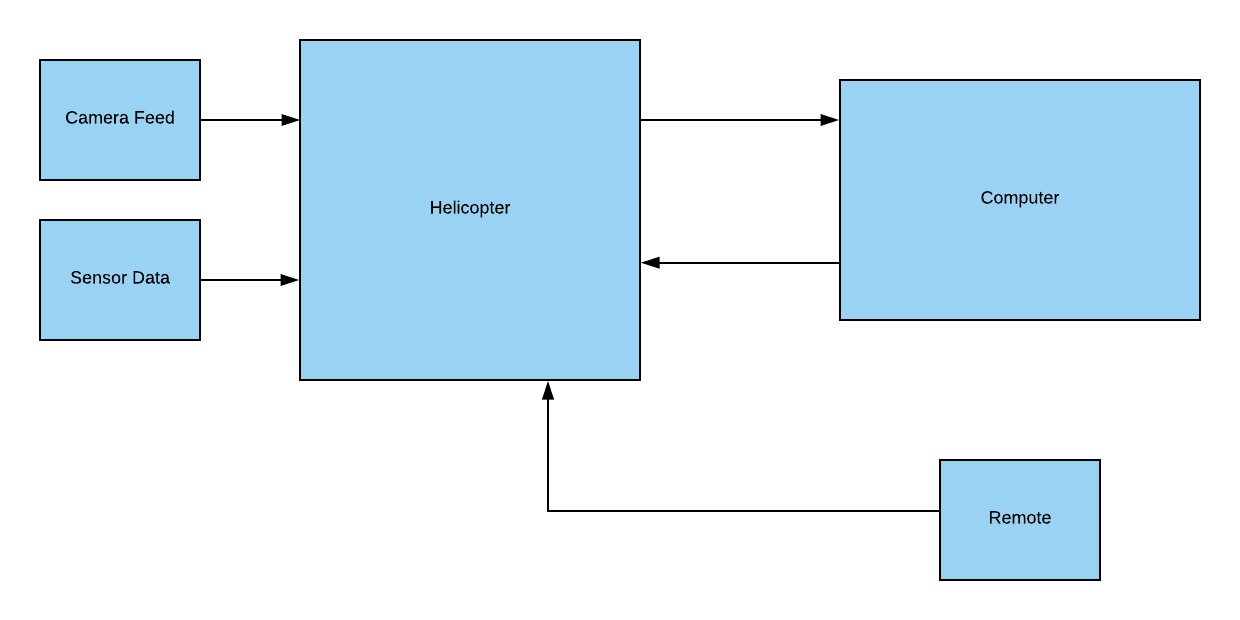
\includegraphics[width=0.7\textwidth]{graphics/high_level_overall_arch.png}
    \caption{Overall System Software Architecture}
    \label{fig:OverallSystemArchitecture}
\end{figure}

\noindent \newline
The responsibilities of the helicopter is to fly through the obstacle course and send data back to the computer. As a part of flying through the course, we want to implement basic collision warning system for the pilot.

\noindent \newline
The computer has the capability to transmit data to the helicopter, but this feature is currently unused as the pilot will solely operate the movement of a helicopter with a remote.

\noindent \newline
The cameras, sensors, and computer are the only external systems that will send information to our helicopter module in the Raspberry Pi. The remote will send signals to the helicopter, but those signals will not be used by any of our modules.

\subsection{Helicopter}
Our helicopter, operated by a Raspberry Pi Zero and will contain software made in part by us, the Computer Science subsection of the team, and the Electrical Engineer subsection of the team. \\

\noindent \newline
The diagram below, figure \ref{fig:HelicopterSoftwareArchitecture}, outlines the intended structure of the helicopter\textquotesingle s software. The Raspberry Pi only receives inputs from various sensors, and computer signals from a Wifi transmitter. Outputs are limited to sending signals to handle motor control, and sending sensor and camera data back to the computer. The collision avoidance blocks are unused by our software, but the hooks are still available on the Raspberry Pi. The block will simply pass the data through without modification. Also, the LEDs and speakers were removed due to weight constraints.

\begin{figure}[h]
    \centering
    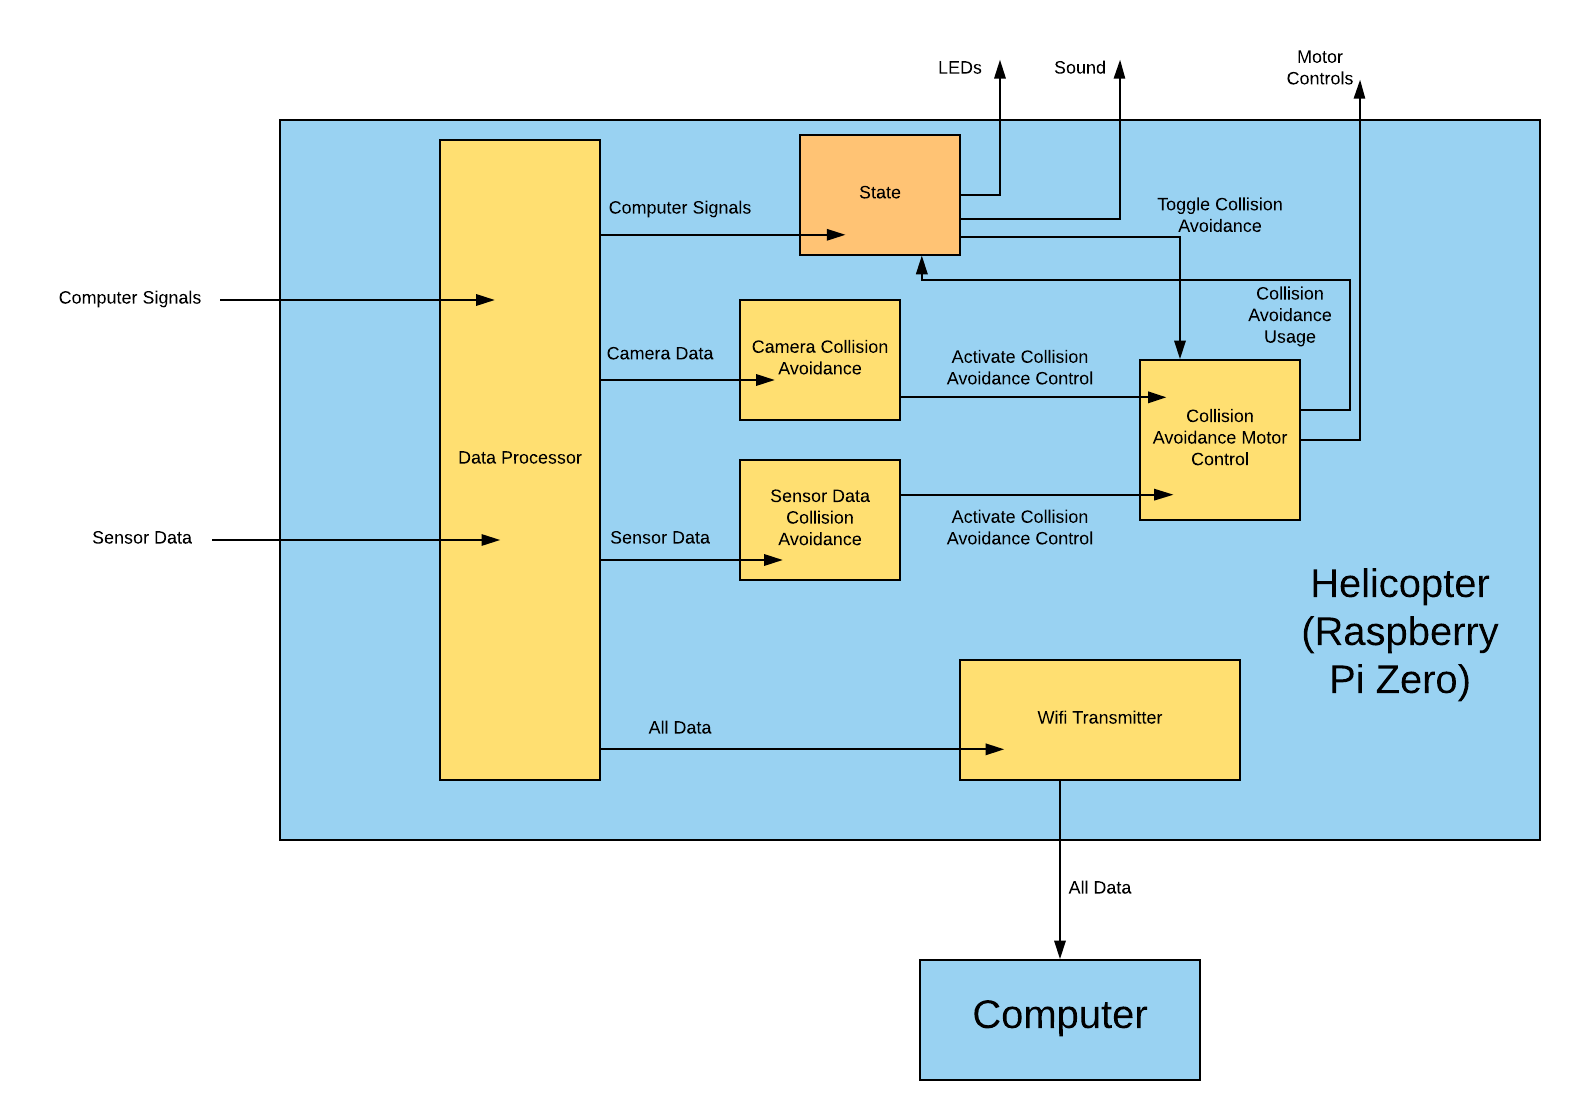
\includegraphics[width=0.9\textwidth]{graphics/helicopter_diagram.png}
    \caption{Helicopter Software Architecture}
    \label{fig:HelicopterSoftwareArchitecture}
\end{figure}

On-board the helicopter, all incoming signals start by entering into a data processing module which ensures that all incoming data is encapsulated in a format the rest of the system can interpret as opposed to possibly a stream of bytes. The data processor is also responsible for keeping the data sorted and outputting the data in an appropriate, timely fashion. The outgoing data will be sent to four different locations, a state module, a collision avoidance module, based on camera data, a collision avoidance module, based on sensor data, and a transmission module which will be responsible of forwarding data on the helicopter to a computer. The state module tracks if the Raspberry Pi has received a proper handshake from the computer and if the Raspberry Pi should be broadcasting or not. It also tracks the orientation, speed, and height of the helicopter and modifies the state based upon sensor inputs.\\

To send the camera feeds and various sensor data to the computer the data processor will send the data to the transmitter module. There the data will be sent to a transmitter through an API provided by the Electrical Engineer subsection of our team.

\subsection{Computer}
Our computer view\textquotesingle s main responsibility is to presenting the camera feeds and flight sensor data to the user. The data coming off the helicopter will be sent to a server running locally on the computer. The server calculates the proper display colors for the collision warning system. The path for the control signals is built, but unused in the software.

\begin{figure}[h]
    \centering
    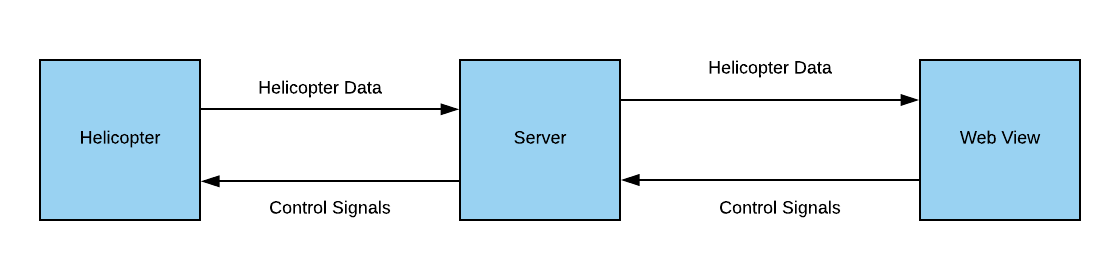
\includegraphics[width=0.8\textwidth]{graphics/computer_diagram.png}
    \caption{Computer View Software Architecture}
    \label{fig:ComputerViewSoftwareArchitecture}
\end{figure}

\section{Component Design}
The following section describes the required software and design components.

\subsection{Collision Warning}
\subsubsection{Introduction}
Collision warning enhances pilot\textquotesingle s awareness of the surroundings, including outside the field of view provided by the camera. To inform the pilot of obstacles surrounding the perimeter of the MAV, we implement a collision warning system.

\subsubsection{Structure}
The system involves three \textit{LV-MaxSonar-EZ0} ultrasonic range sensors, with one at the front and two at the sides of the MAV. Due to the scarcity of available power and an imposed mass limit requirement, a range sensor at the rear of the MAV is not included. The range sensors detect obstacles within a conical-like field of view. Whenever the MAV is close to the ground, there is a chance for the ground itself to be treated as an obstacle. Using a bottom facing range sensor will allow for temporarily turning off collision warning system whenever the MAV is near the surface of the terrain.

\noindent
\newline
Collision warning system is established at the server side. Range sensor data received from the MAV is processed at the server side and reflected in the graphical user interface, as noted in figure \ref{fig:ColWar}. Each pie slice represents the range of the associated ultrasonic range sensor. The range of each ultrasonic sensor, which varies between 6 and 254 inches, is converted to a color. The colors transition from green with the range being the farthest, to yellow with the range being intermediate, and to red with the range being proximal.
\begin{figure}[h]
    \centering
    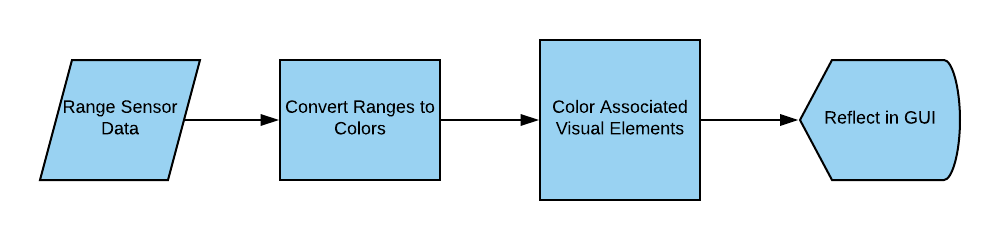
\includegraphics[height=3.5cm]{graphics/collision_warning.png}
    \caption{Collision Warning Flow}
    \label{fig:ColWar}
\end{figure}

\subsubsection{GUI Element}
The GUI consists of a top view of the MAV, surrounded by colored semi-pie sections, shown in figure \ref{fig:ColWarGUI}. Each pie section is dedicated to its associated range sensor and is colored in green, yellow, orange, or red, depending on how far an obstacle is. Red indicates obstacle is too close and green indicates no obstacles within a safe radius.
\begin{figure}[h]
    \centering
    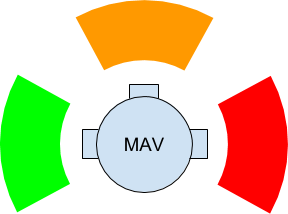
\includegraphics[height=3.5cm]{graphics/collision_warning_gui.png}
    \caption{Collision Warning GUI}
    \label{fig:ColWarGUI}
\end{figure}

\subsubsection{Design Rationale}
The design concept was acquired from the visual display of the road vehicle parking assist software. This allows for the pilot to see where the helicopter is located with respect to obstacles. Additionally, because the field of view of the front facing camera is not wide enough to encapsulate the sides of the MAV, ultrasonic range sensors at the sides of the MAV, to an extent, fulfill missing visual information.

\subsection{Height Indicator}
\subsubsection{Introduction}
Height detection provides GUI feedback for the pilot regarding how high the MAV is from the surface of the terrain.

\subsubsection{Structure}
To inform the pilot of the height, down-facing range sensor is placed at the bottom of the MAV. Range acquired from the down-facing range sensor is transmitted to the server, where it is converted to meters, formatted, and written to a text input element within the GUI.

\subsubsection{GUI Element}
For the pilot to be aware of the height, a label element, \textit{Height}, along with a height value next to the label is included. The height element is positioned at the upper-left corner of the GUI.

\subsubsection{Design Rationale}
When flying over obstacles, a pilot must be aware of the range he is from the obstacle below. For the pilot, being aware of height is especially crucial when landing or flying high and solely relying on the graphical user interface for the vision. Visual input coming from the front and package cameras does provide the pilot with the necessary height awareness; however, measured height improves awareness.

\subsection{Attitude Indicator}
\subsubsection{Introduction}
Vertical alignment awareness allows for the pilot to know how the MAV is aligned with respect to the horizon. There are two components to the vertical alignment: front-tilt and side tilt. Both of the values are represented by the attitude indicator.

\subsubsection{Structure}
Data obtained from the accelerometer is converted to pitch and roll angles and transmitted to the server. The server then reflects the pitch and roll in the attitude indicator.

\subsubsection{GUI Element}
Instead of designing the attitude indicator from scratch, we use an existing jQuery plguin, \textit{Flight Indicators}, by Matton Sébastien. \textit{Flight Indicators} provides a number of flight instruments, including attitude indicator, heading indicator, vertical speed indicator, air speed indicator, and altimeter indicator. The attitude indicator, shown in figure \ref{fig:attitude}, is positioned at the bottom-left corner.

\begin{figure}[h]
    \centering
    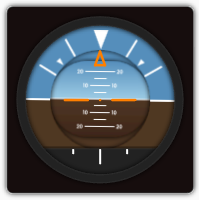
\includegraphics{graphics/attitude.png}
    \caption{Attitude Indicator}
    \label{fig:attitude}
\end{figure}

\subsubsection{Design Rationale}
All manual controlled aviation vehicles have attitude instrument. It is beneficial for the MAV pilot to have access to the vertical alignment data as well.

\subsection{Heading Indicator}
\subsubsection{Introduction}
In addition to the attitude indicator, an awareness of the direction the MAV is facing is, too, be suitable for the pilot. We implement a heading indicator, which is a compass.

\subsubsection{Structure}
Data obtained from the accelerometer is converted to yaw angle and transmitted to the server. The server then reflects the yaw value in the heading indicator.

\subsubsection{GUI Element}
We implement an existing heading indicator provided by the jQuery plguin, \textit{Flight Indicators}. The heading indicator, displayed in figure \ref{fig:heading}, is positioned at the bottom-left corner, next to the attitude indicator.

\begin{figure}[h]
    \centering
    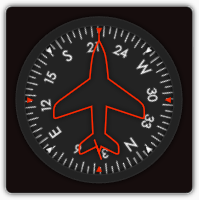
\includegraphics{graphics/heading.png}
    \caption{Attitude Indicator}
    \label{fig:heading}
\end{figure}

\subsubsection{Design Rationale}
When navigating through the competition map, it is convenient for pilot to be aware the direction the MAV is facing. Because heading indicator is not as crucial for the pilot as any of the video feeds, the GUI element accumulates a small area on the screen.

\subsection{Speed Indicator}
\subsubsection{Introduction}
Awareness of the overall velocity of the MAV is, too, useful for the pilot to know. Although speed indicator is not a crucial component, presenting the flight variable to the pilot allows for the pilot to keep track of the velocity.

\subsubsection{Structure}
Linear acceleration values obtained from the accelerometer are integrated with Euler integration, and added to the overall velocity vector. The magnitude of the velocity vector is transmitted to the server and reflected in the text label.

\subsubsection{GUI Element}
The speed label, along with the value, in meters per second, is displayed at the uppler-left corner of the screen.

\subsubsection{Design Rationale}
Presenting speed in text form is enough for the pilot to be aware of how fast the MAV is moving. Additionally, velocity is not an important indicator and must, therefore, acquire minimal area on the main screen.

\subsection{Front Video Feed}
\subsubsection{Introduction}
Front camera video feed is the most essential and a required component of the design.

\subsubsection{GUI Element}
A background window element with video feed overlaying the entire screen.

\subsubsection{Design Rationale}
Because video feed is a required component and allows for the pilot to see what the MAV is doing whenever the MAV is not visible to the pilot, the entire video feed should stand out. Overlaying the entire monitor provides a clear visual display for the pilot.

\subsection{Bottom Video Feed}
\subsubsection{Introduction}
Down facing camera provides additional visual information to the pilot. The down-facing camera is used to assist the pilot in package pickup and provides awareness of obstacles below.

\subsubsection{GUI Element}
A smaller rectangular area at the upper-right corner of the screen, displaying the down-facing camera video feed.

\subsubsection{Design Rational}
Because bottom video feed is not as important as the front video feed, the rectangular area for the bottom video feed must not stand out.

\section{Graphical User Interface}
The graphical user interface consists of a web-page, with the entire background covered with a front view video feed. Flight instrument component elements and bottom facing camera feed element overlay the sides of the main video feed and may be semi-transparent. When package pickup mode is entered, the bottom facing camera feed window is enlarge sightly and pickup guidance elements are presented. Shown in figure \ref{fig:UI1} is a mock-up of the GUI. All GUI elements, except for the flight variables, are explanatory. The flight variables section provides the pilot with height, velocity, forward tilt, and a any other non-essential variables.

\begin{figure}[h]
    \centering
    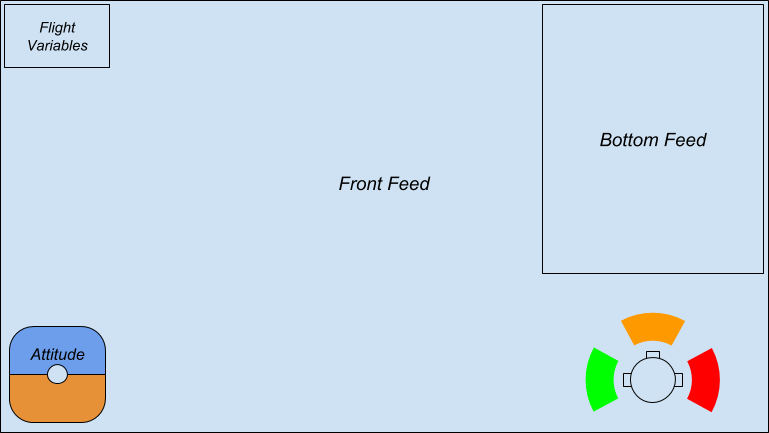
\includegraphics[width=0.9\textwidth]{graphics/ui1.png}
    \caption{Graphical User Interface Mock-up}
    \label{fig:UI1}
\end{figure}

\noindent
\newline
For the actual deign, shown in figure \ref{fig:UI2}, we develop the front feed and bottom feed elements, the collision warning instrument, and the flight variables element. For flight instruments, we found an existing jQuery plugin, \textit{Flight Indicators}. \textit{Flight Indicators} provides a number of flight instruments, including attitude indicator, heading indicator, vertical speed indicator, air speed indicator, and altimeter indicator. We use attitude indicator and heading indicator. Both of these indicators represent the yaw, pitch, and roll of the MAV, based on the values fed from the accelerometer onboard.

\noindent
\newline
The height flight variable displays the range of the down-facing ultrasonic sensor in meters. Making use of the altimeter indicator for displaying the height would have not been suitable as altimeter measures the altitude from the sea level and not the altitude to the terrain below.

\noindent
\newline
The speed flight variable displays the magnitude of the velocity of the helicopter, also obtained from integrating linear acceleration obtained from the accelerometer.

\begin{figure}[h]
    \centering
    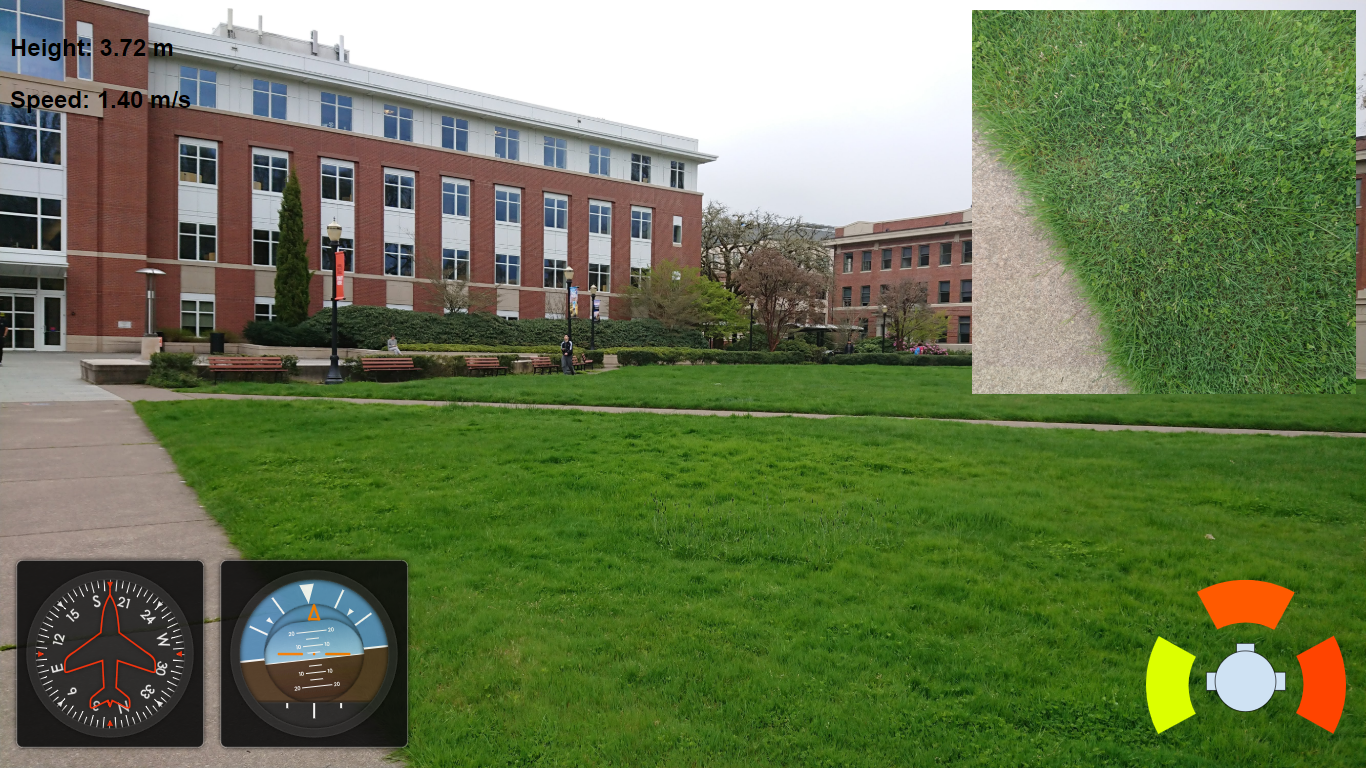
\includegraphics[width=0.9\textwidth]{graphics/ui2.png}
    \caption{Graphical User Interface}
    \label{fig:UI2}
\end{figure}

\noindent
\newline
All the values represented in the GUI are obtained at the Raspberry Pi side, transmitted to the server via UDP, and reflected in the GUI. We currently display artificially generated values for the collision warning instrument, attitude indicator, heading indicator, and the flight variables. For consistency and legitimacy of testing, all the generated values are transmitted from the Raspberry Pi. Both, the front feed and bottom feed, display the actual camera feeds transmitted from the Raspberry Pi. We also implement the ultrasonic sensor for displaying the actual height flight variable. The instructions for using the down facing ultrasonic sensor are documented in the \textit{README} of MAV Senior Capstone repository.

\clearpage
\medskip
\bibliographystyle{IEEEtran}
\bibliography{ref}
\end{document}
